
\section{Programs for Graphical display\index{display} of calculated data}
\label{graphics}

If java is installed on the system, running McPhase will
 display\index{display} the calculated magnetisation
curve immediately during the simulation updating 
it in regular intervals (this can be done for any other
curve  by using the
program: {\prg display\index{display} x-colnr y-colnr filename}). 
Also the text in output files can be monitored by the program:
{\prg displaytext\index{displaytext} filename}.
During the simulation
the results are stored in the directory {\prg ./results}, the output files can be viewed 
using the programs described in this section. 

\subsection{Programs {\prg display},{\prg displaybubbles\index{displaybubbles} },{\prg %%@
displaycontour\index{displaycontour}},{\prg displaytext\index{displaytext}} and {\prg show} - graphical %%@
display\index{display} of any xy data such as magnetisation etc.}
\label{display}

\begin{description} 
\item [display\index{display} 1 11 ./results/mcphas.fum] produces a graphical display\index{display} of the data %%@
file
mcphas.fum on screen. The display\index{display} contains an xy plot of column 1 versus column 11
({\prg java} has to be installed to use this program). 
More files may be displayed by commands such as

{\bf display\index{display} 1 2 data1.dat 3 5 data2.dat}.

Note that viewing of 
data which is generated by programs may be viewed online. The program updates the plot
every 500 milliseconds. In this way it is possible to watch online, how programs
calculate data. The output of display\index{display} may contain lines to tune the display\index{display} output, %%@
such as
\begin{verbatim}
	 #! displayytext=intensity

	 #! displayxtext=meV 

	 #! displaylines=true 

	 #! displaytitle=My new Graph

	 #! displaylegend=false 
\end{verbatim} 

\item [displaybubbles\index{displaybubbles}  5 6 8 ./results/mcdisp.qei] works similar as display, however
a third column is given and the radius of the symbols varied according to the data in 
this column.

\item [displaycontour\index{displaycontour} 5 6 8 ./results/mcdisp.dsigma.tot] produces a graphical
display\index{display} of a 3 dimensional dataset as a colour and/or contour plot. Here '5 6 8' 
denote the x,y and z column in file {\prg ./results/mcdisp.dsigma.tot}, which should
be plotted. Figure~\ref{diffus} shows an sample output of this program.

\item [displaytext\index{displaytext} ./results/mcphas.hkl] monitors the file mcphas.hkl in a text window
on screen.

\item [show 1 11 ./results/mcphas.fum]     produces a gnuplot graphic 
({\prg gnuplot} must be installed
on the system in order to use this).
\end{description} 
the following example shows the temperature dependence of the magnetisation
of NdCu$_2$

\begin{figure}[hb]%h=here, t=top, b=bottom, p=separate figure page
\begin{center}\leavevmode
\includegraphics[angle=-90, width=0.7\textwidth]{figsrc/ndcu2b/resultss/mag0_2T.ps}
\end{center}
\caption{Calculated temperature dependence of the magnetisation  along the crystallographic
$b$-direction  of NdCu$_2$ for an applied magnetic field of 0.2~T 
[plot created by program {\prg show+gnuplot}]}
\label{magnetizationgraphic}
\end{figure}
%\clearpage


\subsection{Program {\prg spins\index{spins}} - display\index{display} of the moment configuration for a given %%@
temperature/field}
\label{spins}

\begin{description} 
\item [spins T Ha Hb Hc [file.sps||file.mf||h k l E(meV)]]       produces plot of spin-configuration at $T-H$ %%@
point
\end{description} 

Note, the graphics output format can be fine tuned in .sps and .qev input filescan be fine tuned in .mf input %%@
files by setting the variables
{\prg show\_abc\_unitcell, show\_primitive\_crystal\_unitcell, show\_magnetic\_unitcell, show\_atoms, %%@
scale\_view\_1,
scale\_view\_2, scale\_view\_3}, and in
the  .qev input file bye setting 
{\prg spins\_wave\_amplitude, spins\_show\_ellipses, spins\_show\_direction\_of\_static\_moment}.

Output files:
\begin{enumerate}
  \item encapsulated postscript ps-file {\prg results/spins*.eps}, 
  \item the files {\prg results/spins.fst} and {\prg results/spins\_prim.fst} are created, 
                which can be read by the fullprof program {\prg fp\_studio}
                for on screen display\index{display} of a spin configuration,
  \item the spin-configuration is printed to stdout - therefore
                               this program can be used with a .mf file 
			       to generate an input file
			       for program {\prg  McDisp} (example: {\prg spins 1 1 0 0 spins.mf $>$ mcdisp.mf})  
  \item the text file {\prg results/spins.out} is created, which is useful to produce input files for
              the diffraction program {\prg mcdiff\index{mcdiff}}
  \item the graphics files {\prg results/spins.jvx} and {\prg results/spins\_prim.jvx}, which can be displayed
         by the program {\prg javaview}, e.g. by the command {\prg java javaview spin\_prim.jvx}.
  \item if {\prg spins} is used with arguments {\prg h k l E(meV)}, it takes the eigenvectors of magnetic %%@
excitations
        from the file {\prg results/mcdisp.qev} (usually created by {\prg mcdisp}) and produces a graphical
        animation of the spin osciallation which is associated with this magnetic mode. The output is a series
        of files {\prg results/spins.*.jvx} and {\prg results/spins\_prim.*.jvx} which can be viewed by program
        {\prg javaview}, e.g. by the command {\prg java javaview "model=results/spins\_prim.*.jvx" 
        Animation.LastKey=16 background="255 255 255"}.  {\prg javaview} is also able to produce a sequence
		of gif files (press c in the animation window), which can then be processed by an animatino editor
		to generate an animation, which can be inserted in presentations. For example, you can use {\prg %%@
Imagemagick}
        to create an animation. The following command will issue a proper gif animation, which you can include in %%@
power point        
        presentations etc.: {\prg convert -delay 1 -size 100x100 -loop 1 geomAnim.*.gif output.gif}.
 \end{enumerate}

\begin{figure}[hb]%h=here, t=top, b=bottom, p=separate figure page
\begin{center}\leavevmode
\includegraphics[angle=0, width=0.5\textwidth]{figsrc/ndcu2b/resultss/spinsab.eps}
\end{center}
\caption{Calculated Spin-Structure of NdCu$_2$ at $T=$~2~K and $H=0$.
[plot created by program {\prg spinsab.eps}]}
\label{spingraphic}
\end{figure}

\subsection{Programs to calculate and display Charge-, Spin-, Moment- and Currentdensities
of the unfilled shell}

\subsubsection{Chargedensity - {\prg display\_chargedensity\index{display\_chargedensity}},
{\prg display\_chargedensities\index{display\_chargedensities}},
{\prg chrgplt\index{chrgplt}} and  {\prg charges\index{charges}} - calculation and display of
the charge density for a given temperature/field}
\label{charges}

\begin{description} 
\item [chrgplt\index{chrgplt}  threshold T Ha Hb Hc [singleion-parameter-file]]
 calculates chargedensity for a single ion at given temperature and magnetic field
\item [display\_chargedensity\index{display\_chargedensity}  threshold T Ha Hb Hc [singleion-parameter-file]]
 calculates the chargedensity for a single ion (using {\prg chrgplt})
 and displays it on screen (using {\prg javaview} and {\prg displaycontour}).
\item [charges threshold T Ha Hb Hc [mcphas.mf||h k l E(meV)]]
 calculates chargedensity for a magnetic unit cell calculated by {\prg mcphas} and
 stored in {\prg mcphas.mf} for a specifc temperature and magnetic field
\item [display\_chargedensities threshold T Ha Hb Hc [mcphas.mf||h k l E(meV)]]
 calculates the chargedensity for a magnetic unit cell (using {\prg charges})
 and displays it on screen (using {\prg javaview} and {\prg displaycontour}).
\end{description}

   For the calculation of the charge density the following formulas are used (see %%@
appendix~\ref{chargedensityoperator} for a derivation), 

(i) for external single ion modules ({\prg ic1ion})
   
  \begin{equation}\label{chargedensity}
	       \langle \hat\rho(\mbf r)\rangle=
	       -|e|  |R(r)|^2 \sum_{l,m}Z_l^{m}(\Omega) \langle\sum_i Z_l^{m}(\Omega_i)\rangle
   \end{equation} 
  
(ii) for module {\prg so1ion} ({\prg cfield})
   
   \begin{equation}\label{chargedensity_operator}
	       \langle \hat\rho(\mbf r)\rangle=|R_{4f}(r)|^2 \sum_{l=0,2,4,6}\sum_{m=-n,...,n}
	       e  c_{nm} \theta_{l} \langle O_l^m(\mbf J)\rangle_T Z_{lm}(\Omega)
	      \end{equation}
		  
For the notation see \cite{hutchings64-227}: the $R_{4f}$ is the radial part of the
4f wave function (in program {\prg charges\index{charges}} this is taken the same for all
rare earth), $e$ the elementary charge, $c_{nm}$ the pre factors of harmonic tesseral
functions $Z_{lm}(\Omega)$ as given in table IV in \cite{hutchings64-227} and in appendix~\ref{tesseral}, %%@
$\Theta_l$
correspond to the number of electrons for $l=0$
 and the Stevens factors $\alpha$,$\beta$ and $\gamma$ for $l=$~2,4,6, respectively.

The program {\prg chrgplt\index{chrgplt}} just calculates the single ion
problem and therefore only uses a single ion parameter file.
{\prg charges\index{charges}} on the other hand requires input files and the result of a
full {\prg mcphas} simulation.

Note, the graphics output format of program {\prg charges} 
can be fine tuned in .mf input files by setting the variables
{\prg show\_abc\_unitcell, show\_primitive\_crystal\_unitcell, show\_magnetic\_unitcell, show\_atoms, %%@
scale\_view\_1,
scale\_view\_2, scale\_view\_3, show\_spindensity, show\_chargedensity}, and in
the  .qee input file bye setting {\prg spins\_wave\_amplitude, spins\_show\_ellipses, %%@
spins\_show\_direction\_of\_static\_moment}.


Output files:
\begin{enumerate}
  \item the charge moments and some information are printed to stdout 
  \item the graphics files {\prg chrgplt\index{chrgplt}.jvx}, {\prg results/charges.jvx} and {\prg %%@
results/charges\_prim.jvx}, which can be displayed
         by the program {\prg javaview}, e.g. by the command {\prg java javaview results/charges\_prim.jvx}.
  \item the files {\prg chrgplt*.grid  charges*.grid} containing the charge density
on a grid. {\prg *i.grid *j.grid *k.grid} contain the charge densities
in three orthogonal planes. {\prg *.grid} contains the full charge density on a
three dimensional grid. Grid parameters can be set in {\prg results/graphic\_parameters.set}.
  \item {\prg charges} produces the text file {\prg results/charges.out} is created, which is useful to produce %%@
input files for
              the diffraction program {\prg mcdiff\index{mcdiff}} in order to go beyond the dipole approximation
              for calculating the neutron form factor.
  \item if {\prg charges} is used with arguments {\prg h k l E(meV)}, it takes the eigenvectors of magnetic %%@
excitations
        from the file {\prg results/mcdisp.qee} (usually created by {\prg mcdisp}) and produces a graphical
        animation of the spin/charge oscillation which is associated with this excitation. The output is a series
        of files {\prg results/charges.*.jvx} and {\prg results/charges\_prim.*.jvx} which can be viewed by %%@
program
        {\prg javaview}, e.g. by the command {\prg java javaview "model=results/charges\_prim.*.jvx" 
        Animation.LastKey=16 background="255 255 255"}.
 \end{enumerate}

\begin{figure}[hb]%h=here, t=top, b=bottom, p=separate figure page
\begin{center}\leavevmode
\includegraphics[angle=0, width=0.7\textwidth]{figsrc/ndcu2b/resultss/chargesab.eps}
\end{center}
\caption{Calculated 4f Charge-Structure of NdCu$_2$ at $T=$~2~K and $H=0$.
[plot created by program {\prg charges+javaview}]}
\label{chargegraphic}
\end{figure}

\subsubsection{Spin-, Moment- and Currentdensities}

currently only available in combination with module {\prg ic1ion\index{ic1ion}}.
Formalism based on \cite{balcar75-1581,balcar89-1}.

Single ion programs:
\begin{description}
\item [spindensplt\index{spindensplt} threshold T Ha Hb Hc [singleion-parameter-file]]
 calculates spindensity for a single ion at given temperature and magnetic field
\item [display\_spindensity\index{display\_spindensity}  threshold T Ha Hb Hc [singleion-parameter-file]]
 calculates the spindensity for a single ion (using {\prg spindensplt})
 and displays it on screen (using {\prg javaview} and {\prg displaycontour}).
\item [orbmomdensplt\index{orbmomdensplt} threshold T Ha Hb Hc [singleion-parameter-file]]
 calculates orbital moment density for a single ion at given temperature and magnetic field
\item [display\_orbmomdensity\index{display\_orbmomdensity}  threshold T Ha Hb Hc [singleion-parameter-file]]
 calculates the orbital moment density for a single ion (using {\prg orbmomdensplt})
 and displays it on screen (using {\prg javaview} and {\prg displaycontour}).
\item [momdensplt\index{momdensplt} threshold T Ha Hb Hc [singleion-parameter-file]]
 calculates total moment density for a single ion at given temperature and magnetic field
\item [display\_momdensity\index{display\_momdensity}  threshold T Ha Hb Hc [singleion-parameter-file]]
 calculates the total moment density for a single ion (using {\prg momdensplt})
 and displays it on screen (using {\prg javaview} and {\prg displaycontour}).
\item [currdensplt\index{currdensplt} threshold T Ha Hb Hc [singleion-parameter-file]]
 calculates spindensity for a single ion at given temperature and magnetic field
\item [display\_currentdensity\index{display\_currentdensity}  threshold T Ha Hb Hc [singleion-parameter-file]]
 calculates the current density for a single ion (using {\prg currdensplt})
 and displays it on screen (using {\prg javaview} and {\prg displaycontour}).

Programs for a magnetic unit cell:
\item [spindensities threshold T Ha Hb Hc [mcphas.mf]]
 calculates spindensity for a magnetic unit cell calculated by {\prg mcphas} and
 stored in {\prg mcphas.mf} for a specifc temperature and magnetic field
\item [display\_spindensities threshold T Ha Hb Hc [mcphas.mf]]
 calculates the spindensity for a magnetic unit cell (using {\prg spindensities})
 and displays it on screen (using {\prg javaview} and {\prg displaycontour}).
\item [orbmomdensities threshold T Ha Hb Hc [mcphas.mf]]
 calculates orbital moment density for a magnetic unit cell calculated by {\prg mcphas} and
 stored in {\prg mcphas.mf} for a specifc temperature and magnetic field
\item [display\_orbmomdensities threshold T Ha Hb Hc [mcphas.mf]]
 calculates the orbital moment 
density for a magnetic unit cell (using {\prg orbmomdensities})
 and displays it on screen (using {\prg javaview} and {\prg displaycontour}).
\item [momdensities threshold T Ha Hb Hc [mcphas.mf]]
 calculates total moment density for a magnetic unit 
cell calculated by {\prg mcphas} and
 stored in {\prg mcphas.mf} for a specifc temperature and magnetic field
\item [display\_momdensities threshold T Ha Hb Hc [mcphas.mf]]
 calculates the total moment density for a magnetic 
unit cell (using {\prg momdensities})
 and displays it on screen (using {\prg javaview} and {\prg displaycontour}).
\item [currdensities threshold T Ha Hb Hc [mcphas.mf]]
 calculates current density for a magnetic unit cell calculated by {\prg mcphas} and
 stored in {\prg mcphas.mf} for a specifc temperature and magnetic field
\item [display\_currentdensities threshold T Ha Hb Hc [mcphas.mf]]
 calculates the current 
density for a magnetic unit cell (using {\prg currdensities})
 and displays it on screen (using {\prg javaview} and {\prg displaycontour}).
\end{description}


\subsection{Program {\prg hkl\index{hkl}}, {\prg hkl2d\index{hkl2d}} and {\prg mcdiff\index{mcdiff}} - graphical %%@
display\index{display} of magnetic diffraction intensity}
\begin{description} 
\item [{{\prg hkl\index{hkl}} [options] [file]} ]                   produces neutron intensity graphic
 and postscript-file {\prg hkl.ps}. {\prg perl} and
{\prg pgplot} must be installed in order to use this program.
 Options are -n (plot reflex number n)
-h (help). If no file is given the program uses file {\prg mcphas.hkl}.
\item [{{\prg hkl2d\index{hkl2d}} [options] [file]} ]   same as {\prg hkl\index{hkl}} but two-dimensional colour %%@
plot of intensity.
\end{description} 
the following example (fig.~\ref{neutintgraphic}) shows the temperature dependence of the neutron intensity
on the different harmonics of NdCu$_2$.

\begin{figure}[htb]%h=here, t=top, b=bottom, p=separate figure page
\begin{center}\leavevmode
\includegraphics[angle=-90, width=0.8\textwidth]{figsrc/ndcu2b/resultss/hkl.ps}
\end{center}
\caption{NdCu$_2$: calculated temperature dependence of magnetic amplitudes of the
main propagation vector and higher harmonics (at zero magnetic field).}
\label{neutintgraphic}
\end{figure}

In addition to the display\index{display} of the temperature dependence there is the
possibility to generate a powder diffraction pattern by the 
program mcdiff~\index{mcdiff}. The 
recommended procedure is to use 

\begin{description}
\item[{\prg spins\index{spins}} T Ha Hb Hc:] to generate a file {\prg spins.out} which
contains the spin configuration, lattice etc. information at a the
desired temperature. Edit this output file and at the beginning
of the file insert some additional information as described in section~\ref{mcdiff}
and rename it to {\prg mcdiff.in}.

Continue by using  the modules
\item[{\prg mcdiff\index{mcdiff}}:] as described in detail in section~\ref{mcdiff} to
generate a list of reflections with the corresponding neutron powder
intensities (file {\prg mcdiff\index{mcdiff}.out}). In order to create a powder pattern 
a further step is required using the program
\item[{\prg convolute\index{convolute}}... mcdiff\index{mcdiff}.out [+options] resolution file:]
  is also described in section~\ref{addprog}. This program convolute\index{convolute}s the
reflection list with a specific resolution function.
\end{description}

\clearpage

\subsection{Program {\prg phased} - graphical display\index{display} of magnetic phase diagrams}
\begin{description}
\item [phased    [file]]       produces graphic of magnetic xy($HT$)-phase diagram [file]. Note that
{\prg perl} and {\prg pgplot} are needed in order to use this program.

Mind that the plot produced is based on the phase number given in {\prg mcphas.xyt}, which may be
different for the ''same'' magnetic structure as mentioned above
(section~\ref{outputfiles}, {\prg mcphas.phs}). It is recommended to check carefully, if
some magnetic structures are physically equal, although numbered with different phase numbers by
the program. If such a case is detected, the phase numbers in {\prg mcphas.xyt} should
be put to the same value in order to be able to identify the stability region in the plot
produced by {\prg phased}.


\end{description}

\begin{figure}[hb]%h=here, t=top, b=bottom, p=separate figure page
\begin{center}\leavevmode
\includegraphics[angle=-90, width=0.5\textwidth]{figsrc/ndcu2b/resultss/phased.ps}
\end{center}
\caption{Calculated magnetic phase diagram of NdCu$_2$ for field parallel to the orthorhombic $b$-direction.}
\label{phasediagramgraphic}
\end{figure}
\clearpage


\subsection{Program {\prg felog} - display\index{display} logged free energy for different moment configurations %%@
at a temperature/field (linux with pgplot grphic library only)}

\begin{description} 
\item [felog]                  produces plot of logged q values in reciprocal
space vs free energy (colours). {\prg pgplot} and {\prg perl} are needed in order
to use this graphical tool.
(Trick: in order to get a quick overview of the
q-vector range covered by the mcphas\index{mcphas} simulation just type {\prg felog ./results/mcphas.qvc})
\end{description} 

\begin{figure}[hb]%h=here, t=top, b=bottom, p=separate figure page
\begin{center}\leavevmode
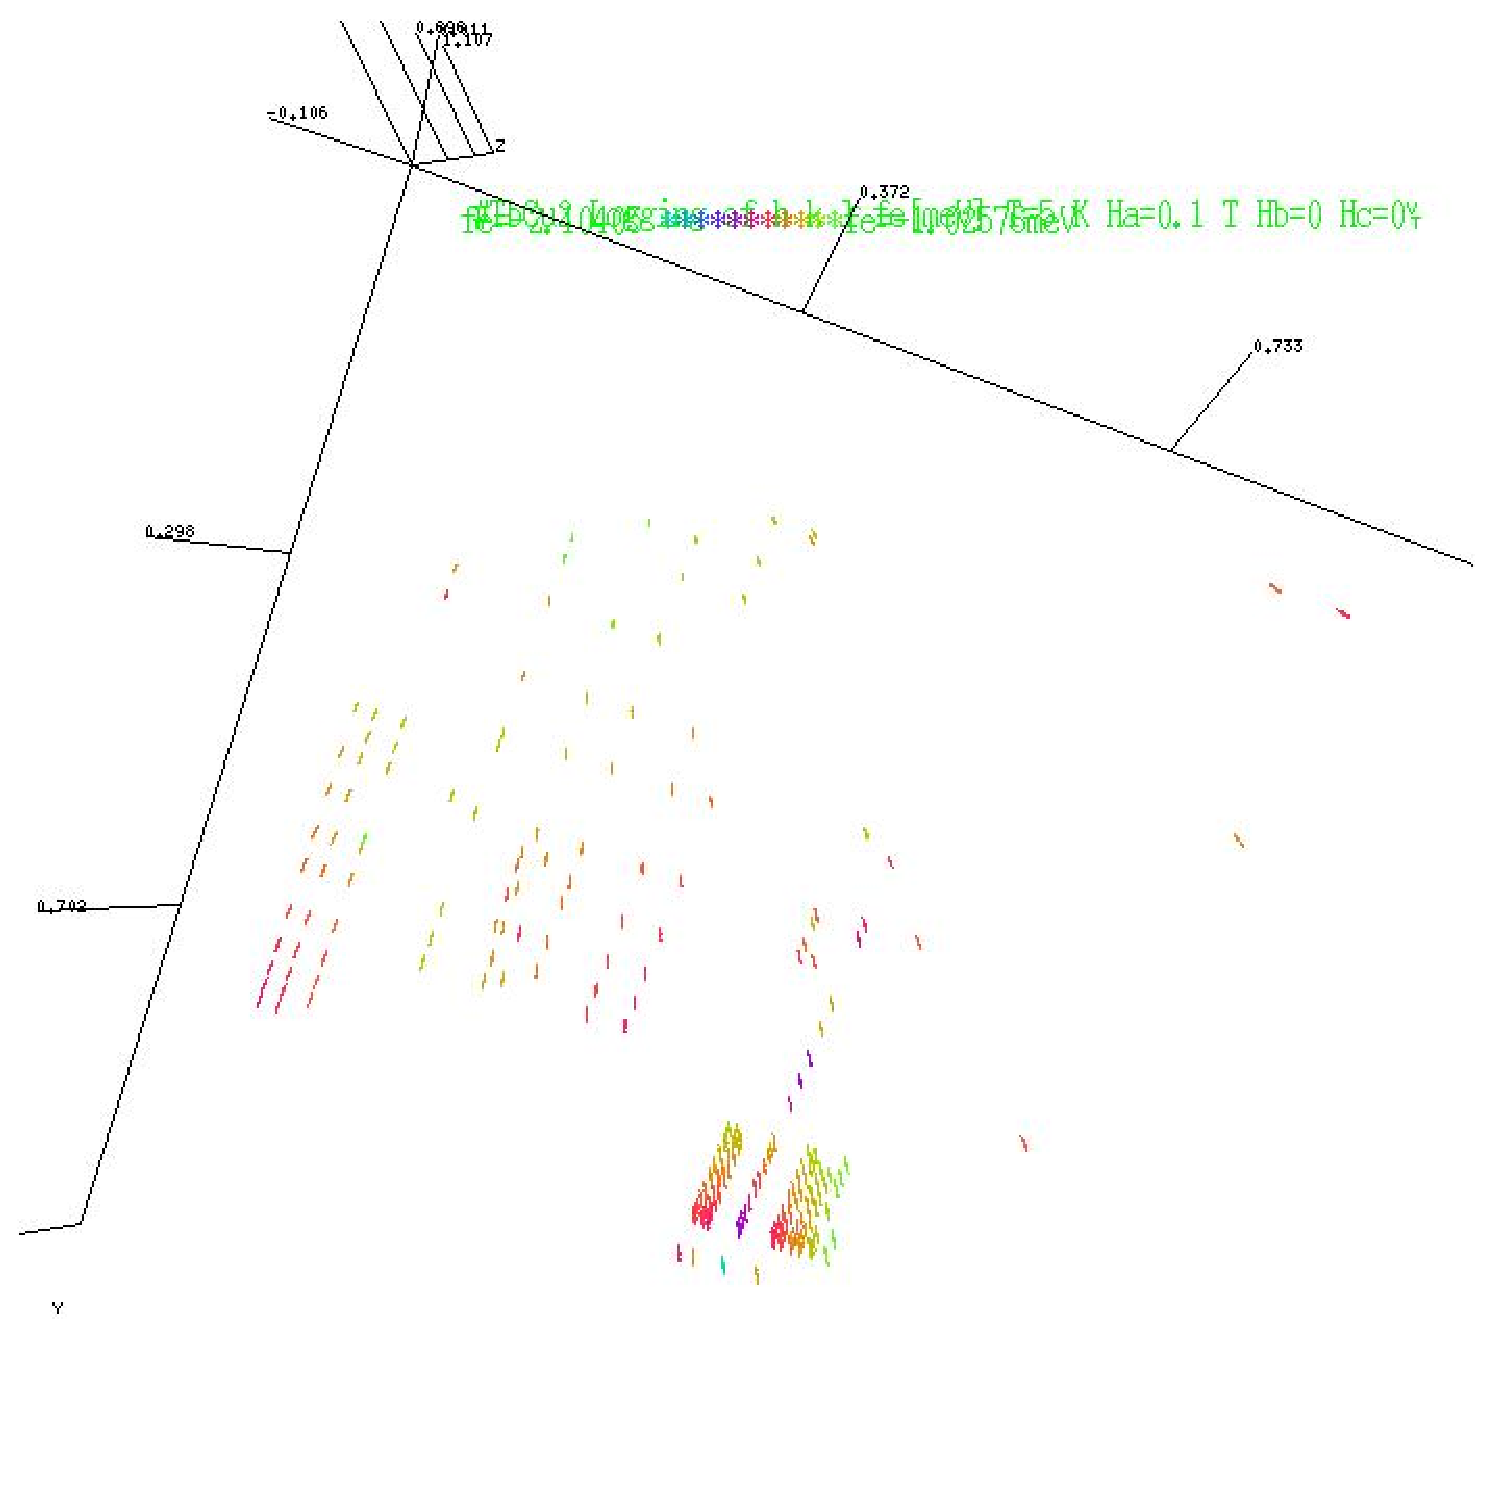
\includegraphics[angle=0, width=0.8\textwidth]{../demo/pictures/felog.eps}
\end{center}
\end{figure}

\vspace{1cm}
{\em Exercises:}
\begin{itemize}
\item Use the programs {\prg phased, hkl, hkl2d, spins, javaview} to generate
graphical output of the simulation results in directory 
{\prg examples/ndcu2b\_new/results}.
\end{itemize}


